\section{Framework}
\label{sec:framework}

Our framework has 4 main components: Path generation, Path searching algorithms, Schedule and Transport and an extra component depicted in Figure \ref{fig:framework}.

\begin{figure}[!htb]
\vspace{-0.1in}
\centering
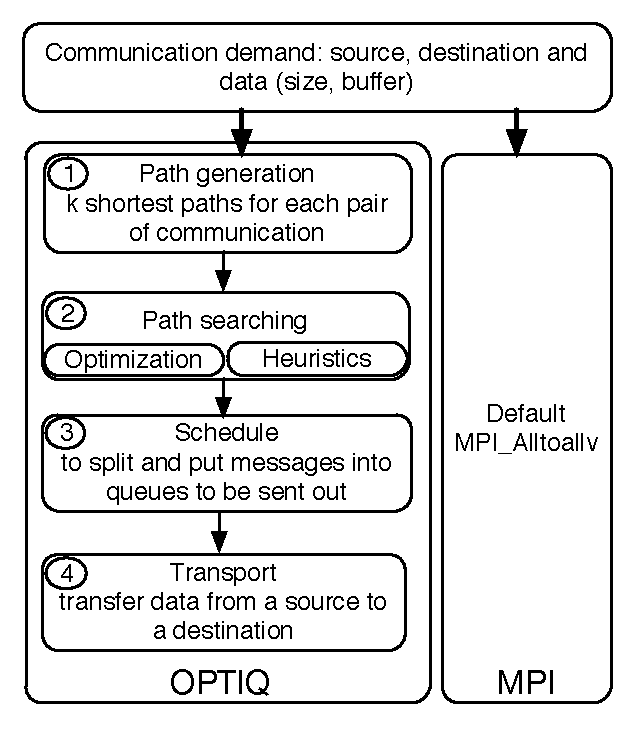
\includegraphics[scale=0.7]{figures/framework.pdf}
\vspace{-0.1in}
\caption{Four components of OPTIQ framework}
\vspace{-0.1in}
\label{fig:framework}
\end{figure}

The functionarity of each component is as following:
\begin{itemize}
\item Path generation: generate k shortest paths that can be used as candidates for data tranfser. We need to generate paths to reduce the search space.
\item Path searching: search for path to transfer data from a set of sources to a set of destination. Multiple or single paths can be found using a set of algorithm. User can decide what algorithm to be used or let the framework use a default algorithm.
\item Schedule: Split a buffer data that needed to tranfer into smaller messages and put those messages into a queue of transport layer to be transferred. It also handles incoming messages for itself and for forwardig them to its neighbors on a way to a message final destination.
As we route data in our own ways, we search for the paths, and we also need to schedule messages transfer. It includes sending local messages, forwarding messages form other sources, receiving data as the intermediate node or the destination node.

Order of messages into sending queue: 3 types of messages: local messages (needed to send), fowarding messages (needed to send), its receiving messages. first come first serve, local messages first. forwa

When there are multiple ranks per node, which one will be choosen to receive data at the next dest (forwarding). Single rank to do or many rank to do, currently every rank executes data transfer.

\item Transport: actually transfer an amount of data from one point to another point in the system.

\end{itemize}

Besides that we have components to get system specific information such as partition size, topology, coordinates, torus, and to compute neighbors of available nodes given to an application. The framework has various options to allow users to tune the framework for optimal performance. For example, the framework allows to select messages from queue to either forward a message from another node first or to send its own message first, to select algorith to search for paths or to set chunk size to transfer a message, to easily add new transport layers on different machine.
